\documentclass{beamer}

\usepackage[cp1252,utf8]{inputenc}
\usepackage[dutch]{babel}
\usepackage{graphicx}
\usepackage{float}
\usepackage{amsmath}
\usepackage{geometry}
%\usepackage{mathtools}
\usepackage{multicol}
\usepackage{amsthm}
\usepackage{amssymb}
\usepackage{algorithm}
\usepackage{geometry}
\usepackage[noend]{algpseudocode}
\usepackage{pgfpages}
\usepackage{listings}
\usepackage{color}


\definecolor{gray}{rgb}{0.5,0.5,0.5}

\lstset{
	frame=tb,
	language=python,
	aboveskip=3mm,
	belowskip=3mm,
	showstringspaces=false,
	columns=flexible,
	basicstyle={\small\ttfamily},
	numbers=none,
	numberstyle=\tiny\color{gray},
	keywordstyle=\color{blue},
	commentstyle=\color{red},
	breaklines=true,
	breakatwhitespace=true,
	tabsize=3
}


\newcommand{\btVFill}{\vskip0pt plus 1filll}

%Information to be included in the title page:
\title{Persoonlijk Project}
\subtitle{Multithreaded Barnes-Hut en Brute force N-body simulatie}
\author{Thomas Van Bogaert}
\date{}

\AtBeginSection[]
{
	\begin{frame}
		\frametitle{}
		\tableofcontents[currentsection]
	\end{frame}
}
\setbeamertemplate{footline}[frame number]
\setbeamertemplate{navigation symbols}{}

%\setbeameroption{show notes}
%\setbeameroption{show notes on second screen=right}

\newcommand{\light}[1]{\textcolor{gray}{#1}}

\begin{document}
	
	\frame{\titlepage}
	\begin{frame}{Wat is een N-body simulatie?}
		\note{
			
		}
		\begin{itemize}
			\item Een simulatie van de werking van krachten tussen verschillende objecten
			\item In het algemeen moet de kracht tussen elk paar objecten berekend worden
			\item Bevoorbeeld: interacties tussen geladen deeltjes of interactie van zwaartekracht tussen sterren
		\end{itemize}
		
	\end{frame}
	
%	\begin{frame}{Waarom een N-body simulatie?}
%		\begin{itemize}
%			\item Verschillende algoritmes beschikbaar (brute force, barnes-hut)
%			\item Goed voorbeeld van een paralleliseerbaar systeem
%		\end{itemize}
%	\end{frame}
	\begin{frame}
			Ik heb het geval van zwaartekracht verder uitgewerkt en twee algoritmes ge\"implementeerd:
			\begin{itemize}
				\item Brute force
				\item Barnes-Hut
			\end{itemize}
			In het implementeren heb ik mij vooral gefocused op performantie
	\end{frame}
	
	\begin{frame}{Uitleg resultaten}
		\note{Vooraleer we naar de resultaten van het brute force algoritme kijken}
		\begin{itemize}
			\item Speedup: Hoeveel keer sneller wordt het algoritme als er meerdere cores gebruikt worden
			\item \b Strong scaling: Voor hoeveel overhead zorgt het parellalisme? Geeft effici\"entie t.o.v. single thread
		\end{itemize}
	\end{frame}
	
	\defverbatim[colored]\codeBF{
		\begin{lstlisting}
		for bodyA in bodies:
			newAcceleration = (0, 0, 0)
			for bodyB in bodies:  # bodyB wordt nooit aangepast
				if bodyA != bodyB:
					forceAB = force(bodyA, bodyB)
					newAcceleration += forceAB / massA
			updateVelocity(bodyA, newAcceleration)
			updateAcceleration(bodyA, newAcceleration)
		\end{lstlisting}
	}
	
	\begin{frame}{Brute force}
		\begin{itemize}
			\item $O(n^2)$
			\item Zeer goed paralleliseerbaar.
		\end{itemize}
		\codeBF
		
	\end{frame}
	
	\begin{frame}{Resultaten Brute Force Multithread: Speedup}
		\begin{center}
			\resizebox{!}{.7\paperheight}{% GNUPLOT: LaTeX picture with Postscript
\begingroup
  % Encoding inside the plot.  In the header of your document, this encoding
  % should to defined, e.g., by using
  % \usepackage[cp1252,<other encodings>]{inputenc}
  \inputencoding{cp1252}%
  \makeatletter
  \providecommand\color[2][]{%
    \GenericError{(gnuplot) \space\space\space\@spaces}{%
      Package color not loaded in conjunction with
      terminal option `colourtext'%
    }{See the gnuplot documentation for explanation.%
    }{Either use 'blacktext' in gnuplot or load the package
      color.sty in LaTeX.}%
    \renewcommand\color[2][]{}%
  }%
  \providecommand\includegraphics[2][]{%
    \GenericError{(gnuplot) \space\space\space\@spaces}{%
      Package graphicx or graphics not loaded%
    }{See the gnuplot documentation for explanation.%
    }{The gnuplot epslatex terminal needs graphicx.sty or graphics.sty.}%
    \renewcommand\includegraphics[2][]{}%
  }%
  \providecommand\rotatebox[2]{#2}%
  \@ifundefined{ifGPcolor}{%
    \newif\ifGPcolor
    \GPcolorfalse
  }{}%
  \@ifundefined{ifGPblacktext}{%
    \newif\ifGPblacktext
    \GPblacktexttrue
  }{}%
  % define a \g@addto@macro without @ in the name:
  \let\gplgaddtomacro\g@addto@macro
  % define empty templates for all commands taking text:
  \gdef\gplbacktext{}%
  \gdef\gplfronttext{}%
  \makeatother
  \ifGPblacktext
    % no textcolor at all
    \def\colorrgb#1{}%
    \def\colorgray#1{}%
  \else
    % gray or color?
    \ifGPcolor
      \def\colorrgb#1{\color[rgb]{#1}}%
      \def\colorgray#1{\color[gray]{#1}}%
      \expandafter\def\csname LTw\endcsname{\color{white}}%
      \expandafter\def\csname LTb\endcsname{\color{black}}%
      \expandafter\def\csname LTa\endcsname{\color{black}}%
      \expandafter\def\csname LT0\endcsname{\color[rgb]{1,0,0}}%
      \expandafter\def\csname LT1\endcsname{\color[rgb]{0,1,0}}%
      \expandafter\def\csname LT2\endcsname{\color[rgb]{0,0,1}}%
      \expandafter\def\csname LT3\endcsname{\color[rgb]{1,0,1}}%
      \expandafter\def\csname LT4\endcsname{\color[rgb]{0,1,1}}%
      \expandafter\def\csname LT5\endcsname{\color[rgb]{1,1,0}}%
      \expandafter\def\csname LT6\endcsname{\color[rgb]{0,0,0}}%
      \expandafter\def\csname LT7\endcsname{\color[rgb]{1,0.3,0}}%
      \expandafter\def\csname LT8\endcsname{\color[rgb]{0.5,0.5,0.5}}%
    \else
      % gray
      \def\colorrgb#1{\color{black}}%
      \def\colorgray#1{\color[gray]{#1}}%
      \expandafter\def\csname LTw\endcsname{\color{white}}%
      \expandafter\def\csname LTb\endcsname{\color{black}}%
      \expandafter\def\csname LTa\endcsname{\color{black}}%
      \expandafter\def\csname LT0\endcsname{\color{black}}%
      \expandafter\def\csname LT1\endcsname{\color{black}}%
      \expandafter\def\csname LT2\endcsname{\color{black}}%
      \expandafter\def\csname LT3\endcsname{\color{black}}%
      \expandafter\def\csname LT4\endcsname{\color{black}}%
      \expandafter\def\csname LT5\endcsname{\color{black}}%
      \expandafter\def\csname LT6\endcsname{\color{black}}%
      \expandafter\def\csname LT7\endcsname{\color{black}}%
      \expandafter\def\csname LT8\endcsname{\color{black}}%
    \fi
  \fi
    \setlength{\unitlength}{0.0500bp}%
    \ifx\gptboxheight\undefined%
      \newlength{\gptboxheight}%
      \newlength{\gptboxwidth}%
      \newsavebox{\gptboxtext}%
    \fi%
    \setlength{\fboxrule}{0.5pt}%
    \setlength{\fboxsep}{1pt}%
\begin{picture}(7200.00,5040.00)%
    \gplgaddtomacro\gplbacktext{%
      \csname LTb\endcsname%%
      \put(946,704){\makebox(0,0)[r]{\strut{}$0.25$}}%
      \csname LTb\endcsname%%
      \put(946,1439){\makebox(0,0)[r]{\strut{}$0.5$}}%
      \csname LTb\endcsname%%
      \put(946,2174){\makebox(0,0)[r]{\strut{}$1$}}%
      \csname LTb\endcsname%%
      \put(946,2909){\makebox(0,0)[r]{\strut{}$2$}}%
      \csname LTb\endcsname%%
      \put(946,3644){\makebox(0,0)[r]{\strut{}$4$}}%
      \csname LTb\endcsname%%
      \put(946,4379){\makebox(0,0)[r]{\strut{}$8$}}%
      \csname LTb\endcsname%%
      \put(1316,484){\makebox(0,0){\strut{}$64$}}%
      \csname LTb\endcsname%%
      \put(2461,484){\makebox(0,0){\strut{}$256$}}%
      \csname LTb\endcsname%%
      \put(3606,484){\makebox(0,0){\strut{}$1024$}}%
      \csname LTb\endcsname%%
      \put(4751,484){\makebox(0,0){\strut{}$4096$}}%
      \csname LTb\endcsname%%
      \put(5896,484){\makebox(0,0){\strut{}$16384$}}%
    }%
    \gplgaddtomacro\gplfronttext{%
      \csname LTb\endcsname%%
      \put(396,2541){\rotatebox{-270}{\makebox(0,0){\strut{}Speedup}}}%
      \put(3940,154){\makebox(0,0){\strut{}# bodies}}%
      \csname LTb\endcsname%%
      \put(2002,4867){\makebox(0,0)[r]{\strut{}1 core}}%
      \csname LTb\endcsname%%
      \put(2002,4647){\makebox(0,0)[r]{\strut{}2 cores}}%
      \csname LTb\endcsname%%
      \put(3781,4867){\makebox(0,0)[r]{\strut{}3 cores}}%
      \csname LTb\endcsname%%
      \put(3781,4647){\makebox(0,0)[r]{\strut{}4 cores}}%
      \csname LTb\endcsname%%
      \put(5560,4867){\makebox(0,0)[r]{\strut{}5 cores}}%
      \csname LTb\endcsname%%
      \put(5560,4647){\makebox(0,0)[r]{\strut{}6 cores}}%
    }%
    \gplbacktext
    \put(0,0){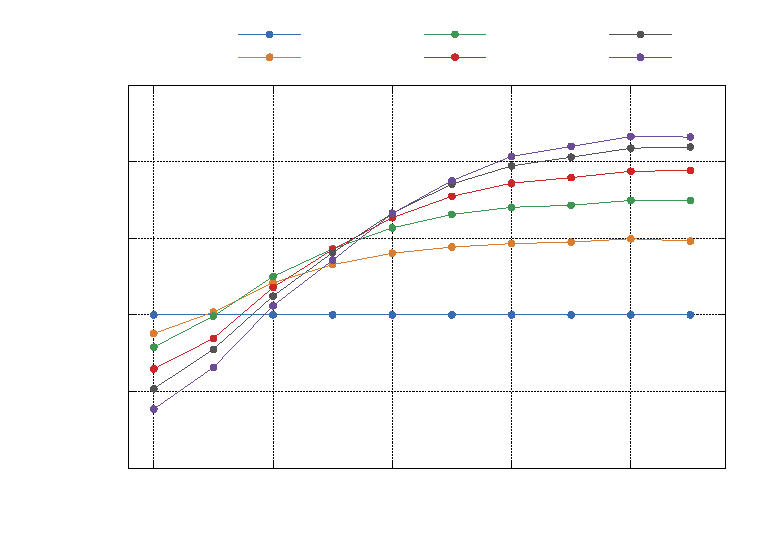
\includegraphics{BFMTSpeedup}}%
    \gplfronttext
  \end{picture}%
\endgroup
}
		\end{center}
	\end{frame}

	
	\begin{frame}{Resultaten Brute Force Multithread: Strong scaling}
		\begin{center}
			\resizebox{!}{.7\paperheight}{% GNUPLOT: LaTeX picture with Postscript
\begingroup
  % Encoding inside the plot.  In the header of your document, this encoding
  % should to defined, e.g., by using
  % \usepackage[cp1252,<other encodings>]{inputenc}
  \inputencoding{cp1252}%
  \makeatletter
  \providecommand\color[2][]{%
    \GenericError{(gnuplot) \space\space\space\@spaces}{%
      Package color not loaded in conjunction with
      terminal option `colourtext'%
    }{See the gnuplot documentation for explanation.%
    }{Either use 'blacktext' in gnuplot or load the package
      color.sty in LaTeX.}%
    \renewcommand\color[2][]{}%
  }%
  \providecommand\includegraphics[2][]{%
    \GenericError{(gnuplot) \space\space\space\@spaces}{%
      Package graphicx or graphics not loaded%
    }{See the gnuplot documentation for explanation.%
    }{The gnuplot epslatex terminal needs graphicx.sty or graphics.sty.}%
    \renewcommand\includegraphics[2][]{}%
  }%
  \providecommand\rotatebox[2]{#2}%
  \@ifundefined{ifGPcolor}{%
    \newif\ifGPcolor
    \GPcolorfalse
  }{}%
  \@ifundefined{ifGPblacktext}{%
    \newif\ifGPblacktext
    \GPblacktexttrue
  }{}%
  % define a \g@addto@macro without @ in the name:
  \let\gplgaddtomacro\g@addto@macro
  % define empty templates for all commands taking text:
  \gdef\gplbacktext{}%
  \gdef\gplfronttext{}%
  \makeatother
  \ifGPblacktext
    % no textcolor at all
    \def\colorrgb#1{}%
    \def\colorgray#1{}%
  \else
    % gray or color?
    \ifGPcolor
      \def\colorrgb#1{\color[rgb]{#1}}%
      \def\colorgray#1{\color[gray]{#1}}%
      \expandafter\def\csname LTw\endcsname{\color{white}}%
      \expandafter\def\csname LTb\endcsname{\color{black}}%
      \expandafter\def\csname LTa\endcsname{\color{black}}%
      \expandafter\def\csname LT0\endcsname{\color[rgb]{1,0,0}}%
      \expandafter\def\csname LT1\endcsname{\color[rgb]{0,1,0}}%
      \expandafter\def\csname LT2\endcsname{\color[rgb]{0,0,1}}%
      \expandafter\def\csname LT3\endcsname{\color[rgb]{1,0,1}}%
      \expandafter\def\csname LT4\endcsname{\color[rgb]{0,1,1}}%
      \expandafter\def\csname LT5\endcsname{\color[rgb]{1,1,0}}%
      \expandafter\def\csname LT6\endcsname{\color[rgb]{0,0,0}}%
      \expandafter\def\csname LT7\endcsname{\color[rgb]{1,0.3,0}}%
      \expandafter\def\csname LT8\endcsname{\color[rgb]{0.5,0.5,0.5}}%
    \else
      % gray
      \def\colorrgb#1{\color{black}}%
      \def\colorgray#1{\color[gray]{#1}}%
      \expandafter\def\csname LTw\endcsname{\color{white}}%
      \expandafter\def\csname LTb\endcsname{\color{black}}%
      \expandafter\def\csname LTa\endcsname{\color{black}}%
      \expandafter\def\csname LT0\endcsname{\color{black}}%
      \expandafter\def\csname LT1\endcsname{\color{black}}%
      \expandafter\def\csname LT2\endcsname{\color{black}}%
      \expandafter\def\csname LT3\endcsname{\color{black}}%
      \expandafter\def\csname LT4\endcsname{\color{black}}%
      \expandafter\def\csname LT5\endcsname{\color{black}}%
      \expandafter\def\csname LT6\endcsname{\color{black}}%
      \expandafter\def\csname LT7\endcsname{\color{black}}%
      \expandafter\def\csname LT8\endcsname{\color{black}}%
    \fi
  \fi
    \setlength{\unitlength}{0.0500bp}%
    \ifx\gptboxheight\undefined%
      \newlength{\gptboxheight}%
      \newlength{\gptboxwidth}%
      \newsavebox{\gptboxtext}%
    \fi%
    \setlength{\fboxrule}{0.5pt}%
    \setlength{\fboxsep}{1pt}%
\begin{picture}(7200.00,5040.00)%
    \gplgaddtomacro\gplbacktext{%
      \csname LTb\endcsname%%
      \put(814,704){\makebox(0,0)[r]{\strut{}$0$}}%
      \csname LTb\endcsname%%
      \put(814,1372){\makebox(0,0)[r]{\strut{}$0.2$}}%
      \csname LTb\endcsname%%
      \put(814,2040){\makebox(0,0)[r]{\strut{}$0.4$}}%
      \csname LTb\endcsname%%
      \put(814,2709){\makebox(0,0)[r]{\strut{}$0.6$}}%
      \csname LTb\endcsname%%
      \put(814,3377){\makebox(0,0)[r]{\strut{}$0.8$}}%
      \csname LTb\endcsname%%
      \put(814,4045){\makebox(0,0)[r]{\strut{}$1$}}%
      \csname LTb\endcsname%%
      \put(946,484){\makebox(0,0){\strut{}$1$}}%
      \csname LTb\endcsname%%
      \put(2117,484){\makebox(0,0){\strut{}$2$}}%
      \csname LTb\endcsname%%
      \put(3289,484){\makebox(0,0){\strut{}$3$}}%
      \csname LTb\endcsname%%
      \put(4460,484){\makebox(0,0){\strut{}$4$}}%
      \csname LTb\endcsname%%
      \put(5632,484){\makebox(0,0){\strut{}$5$}}%
      \csname LTb\endcsname%%
      \put(6803,484){\makebox(0,0){\strut{}$6$}}%
    }%
    \gplgaddtomacro\gplfronttext{%
      \csname LTb\endcsname%%
      \put(396,2541){\rotatebox{-270}{\makebox(0,0){\strut{}effici\"entie}}}%
      \put(3874,154){\makebox(0,0){\strut{}# cores}}%
      \csname LTb\endcsname%%
      \put(2530,4867){\makebox(0,0)[r]{\strut{}4096 bodies}}%
      \csname LTb\endcsname%%
      \put(2530,4647){\makebox(0,0)[r]{\strut{}8192 bodies}}%
      \csname LTb\endcsname%%
      \put(4969,4867){\makebox(0,0)[r]{\strut{}16384 bodies}}%
      \csname LTb\endcsname%%
      \put(4969,4647){\makebox(0,0)[r]{\strut{}32768 bodies}}%
    }%
    \gplbacktext
    \put(0,0){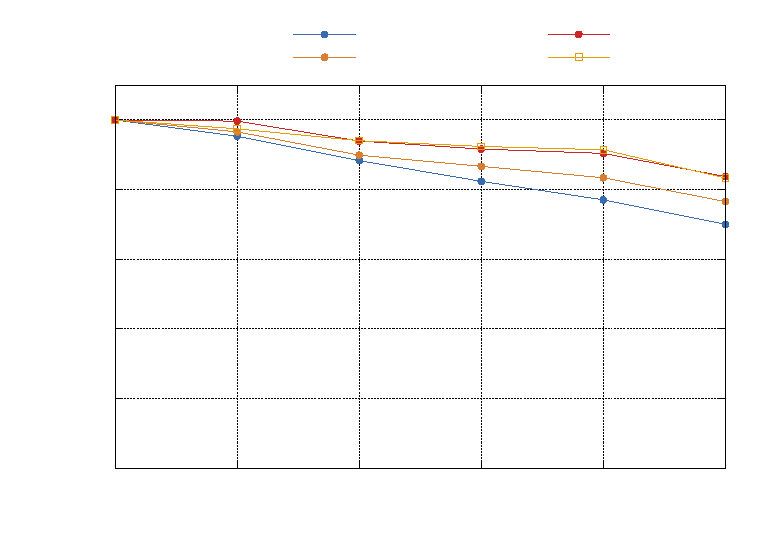
\includegraphics{BFStrong}}%
    \gplfronttext
  \end{picture}%
\endgroup
}
		\end{center}
	\end{frame}
	
	\begin{frame}{Resultaten Brute Force GPU: Speedup}
		\begin{center}
			\resizebox{!}{.7\paperheight}{% GNUPLOT: LaTeX picture with Postscript
\begingroup
  % Encoding inside the plot.  In the header of your document, this encoding
  % should to defined, e.g., by using
  % \usepackage[cp1252,<other encodings>]{inputenc}
  \inputencoding{cp1252}%
  \makeatletter
  \providecommand\color[2][]{%
    \GenericError{(gnuplot) \space\space\space\@spaces}{%
      Package color not loaded in conjunction with
      terminal option `colourtext'%
    }{See the gnuplot documentation for explanation.%
    }{Either use 'blacktext' in gnuplot or load the package
      color.sty in LaTeX.}%
    \renewcommand\color[2][]{}%
  }%
  \providecommand\includegraphics[2][]{%
    \GenericError{(gnuplot) \space\space\space\@spaces}{%
      Package graphicx or graphics not loaded%
    }{See the gnuplot documentation for explanation.%
    }{The gnuplot epslatex terminal needs graphicx.sty or graphics.sty.}%
    \renewcommand\includegraphics[2][]{}%
  }%
  \providecommand\rotatebox[2]{#2}%
  \@ifundefined{ifGPcolor}{%
    \newif\ifGPcolor
    \GPcolorfalse
  }{}%
  \@ifundefined{ifGPblacktext}{%
    \newif\ifGPblacktext
    \GPblacktexttrue
  }{}%
  % define a \g@addto@macro without @ in the name:
  \let\gplgaddtomacro\g@addto@macro
  % define empty templates for all commands taking text:
  \gdef\gplbacktext{}%
  \gdef\gplfronttext{}%
  \makeatother
  \ifGPblacktext
    % no textcolor at all
    \def\colorrgb#1{}%
    \def\colorgray#1{}%
  \else
    % gray or color?
    \ifGPcolor
      \def\colorrgb#1{\color[rgb]{#1}}%
      \def\colorgray#1{\color[gray]{#1}}%
      \expandafter\def\csname LTw\endcsname{\color{white}}%
      \expandafter\def\csname LTb\endcsname{\color{black}}%
      \expandafter\def\csname LTa\endcsname{\color{black}}%
      \expandafter\def\csname LT0\endcsname{\color[rgb]{1,0,0}}%
      \expandafter\def\csname LT1\endcsname{\color[rgb]{0,1,0}}%
      \expandafter\def\csname LT2\endcsname{\color[rgb]{0,0,1}}%
      \expandafter\def\csname LT3\endcsname{\color[rgb]{1,0,1}}%
      \expandafter\def\csname LT4\endcsname{\color[rgb]{0,1,1}}%
      \expandafter\def\csname LT5\endcsname{\color[rgb]{1,1,0}}%
      \expandafter\def\csname LT6\endcsname{\color[rgb]{0,0,0}}%
      \expandafter\def\csname LT7\endcsname{\color[rgb]{1,0.3,0}}%
      \expandafter\def\csname LT8\endcsname{\color[rgb]{0.5,0.5,0.5}}%
    \else
      % gray
      \def\colorrgb#1{\color{black}}%
      \def\colorgray#1{\color[gray]{#1}}%
      \expandafter\def\csname LTw\endcsname{\color{white}}%
      \expandafter\def\csname LTb\endcsname{\color{black}}%
      \expandafter\def\csname LTa\endcsname{\color{black}}%
      \expandafter\def\csname LT0\endcsname{\color{black}}%
      \expandafter\def\csname LT1\endcsname{\color{black}}%
      \expandafter\def\csname LT2\endcsname{\color{black}}%
      \expandafter\def\csname LT3\endcsname{\color{black}}%
      \expandafter\def\csname LT4\endcsname{\color{black}}%
      \expandafter\def\csname LT5\endcsname{\color{black}}%
      \expandafter\def\csname LT6\endcsname{\color{black}}%
      \expandafter\def\csname LT7\endcsname{\color{black}}%
      \expandafter\def\csname LT8\endcsname{\color{black}}%
    \fi
  \fi
    \setlength{\unitlength}{0.0500bp}%
    \ifx\gptboxheight\undefined%
      \newlength{\gptboxheight}%
      \newlength{\gptboxwidth}%
      \newsavebox{\gptboxtext}%
    \fi%
    \setlength{\fboxrule}{0.5pt}%
    \setlength{\fboxsep}{1pt}%
\begin{picture}(7200.00,5040.00)%
    \gplgaddtomacro\gplbacktext{%
      \csname LTb\endcsname%%
      \put(1342,704){\makebox(0,0)[r]{\strut{}$0.03125$}}%
      \csname LTb\endcsname%%
      \put(1342,1132){\makebox(0,0)[r]{\strut{}$0.0625$}}%
      \csname LTb\endcsname%%
      \put(1342,1560){\makebox(0,0)[r]{\strut{}$0.125$}}%
      \csname LTb\endcsname%%
      \put(1342,1988){\makebox(0,0)[r]{\strut{}$0.25$}}%
      \csname LTb\endcsname%%
      \put(1342,2416){\makebox(0,0)[r]{\strut{}$0.5$}}%
      \csname LTb\endcsname%%
      \put(1342,2844){\makebox(0,0)[r]{\strut{}$1$}}%
      \csname LTb\endcsname%%
      \put(1342,3272){\makebox(0,0)[r]{\strut{}$2$}}%
      \csname LTb\endcsname%%
      \put(1342,3701){\makebox(0,0)[r]{\strut{}$4$}}%
      \csname LTb\endcsname%%
      \put(1342,4129){\makebox(0,0)[r]{\strut{}$8$}}%
      \csname LTb\endcsname%%
      \put(1695,484){\makebox(0,0){\strut{}$64$}}%
      \csname LTb\endcsname%%
      \put(2761,484){\makebox(0,0){\strut{}$256$}}%
      \csname LTb\endcsname%%
      \put(3827,484){\makebox(0,0){\strut{}$1024$}}%
      \csname LTb\endcsname%%
      \put(4893,484){\makebox(0,0){\strut{}$4096$}}%
      \csname LTb\endcsname%%
      \put(5958,484){\makebox(0,0){\strut{}$16384$}}%
    }%
    \gplgaddtomacro\gplfronttext{%
      \csname LTb\endcsname%%
      \put(396,2541){\rotatebox{-270}{\makebox(0,0){\strut{}Speedup}}}%
      \put(4138,154){\makebox(0,0){\strut{}# bodies}}%
      \csname LTb\endcsname%%
      \put(3190,4867){\makebox(0,0)[r]{\strut{}1 thread CPU}}%
      \csname LTb\endcsname%%
      \put(3190,4647){\makebox(0,0)[r]{\strut{}6 threads CPU}}%
      \csname LTb\endcsname%%
      \put(5761,4867){\makebox(0,0)[r]{\strut{}GPU Offload}}%
    }%
    \gplbacktext
    \put(0,0){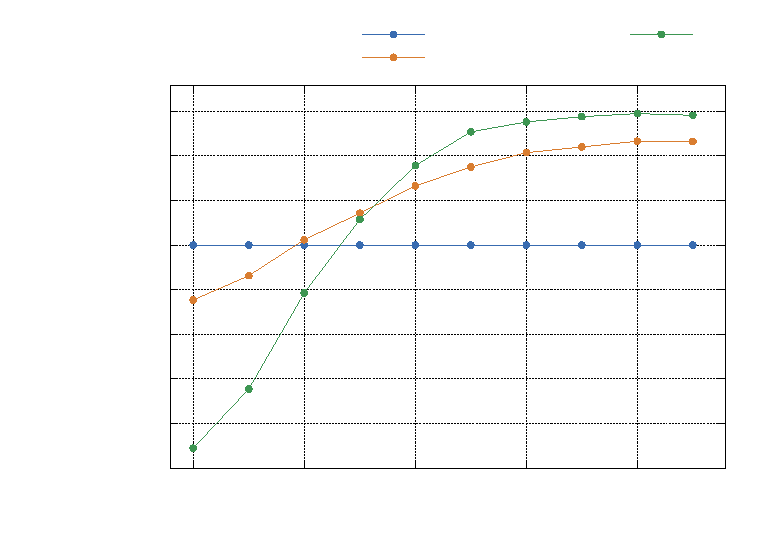
\includegraphics{BFOSpeedup}}%
    \gplfronttext
  \end{picture}%
\endgroup
}
		\end{center}
	\end{frame}

	\defverbatim[colored]\codeBH{
		\begin{lstlisting}
		for body in bodies:
			# traverses tree
			newAcceleration = calculateAcceleration(body, root)  
			updateVelocity(bodyA, newAcceleration)
			updateAcceleration(bodyA, newAcceleration)
		\end{lstlisting}
	}

	\begin{frame}{Barnes-Hut}
		\note{
			
		}
		\begin{itemize}
			\item $O(n log(n))$
			\item Deelt lichamen onder in octree
			\item Het is niet nodig om krachten tussen elk paar lichamen te berekenen.
			
			 Schat verafgelegen lichamen af door het massacentrum
			
			\item Twee implementaties
			\begin{itemize}
				\item Iteratief gebruikmakend van space filling curve
				\item Recursief
			\end{itemize}
		\end{itemize}
		\codeBH
	\end{frame}
	
	\begin{frame}{Barnes-Hut algoritme}
		\begin{center}
			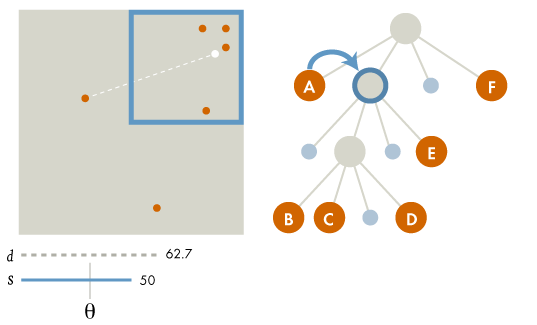
\includegraphics[width= 0.8\linewidth]{quadTreeBH.png}
		\end{center}
	\end{frame}

	\begin{frame}{Resultaten Barnes-Hut Multithread: Speedup}
		\begin{center}
			\resizebox{!}{.7\paperheight}{% GNUPLOT: LaTeX picture with Postscript
\begingroup
  % Encoding inside the plot.  In the header of your document, this encoding
  % should to defined, e.g., by using
  % \usepackage[cp1252,<other encodings>]{inputenc}
  \inputencoding{cp1252}%
  \makeatletter
  \providecommand\color[2][]{%
    \GenericError{(gnuplot) \space\space\space\@spaces}{%
      Package color not loaded in conjunction with
      terminal option `colourtext'%
    }{See the gnuplot documentation for explanation.%
    }{Either use 'blacktext' in gnuplot or load the package
      color.sty in LaTeX.}%
    \renewcommand\color[2][]{}%
  }%
  \providecommand\includegraphics[2][]{%
    \GenericError{(gnuplot) \space\space\space\@spaces}{%
      Package graphicx or graphics not loaded%
    }{See the gnuplot documentation for explanation.%
    }{The gnuplot epslatex terminal needs graphicx.sty or graphics.sty.}%
    \renewcommand\includegraphics[2][]{}%
  }%
  \providecommand\rotatebox[2]{#2}%
  \@ifundefined{ifGPcolor}{%
    \newif\ifGPcolor
    \GPcolorfalse
  }{}%
  \@ifundefined{ifGPblacktext}{%
    \newif\ifGPblacktext
    \GPblacktexttrue
  }{}%
  % define a \g@addto@macro without @ in the name:
  \let\gplgaddtomacro\g@addto@macro
  % define empty templates for all commands taking text:
  \gdef\gplbacktext{}%
  \gdef\gplfronttext{}%
  \makeatother
  \ifGPblacktext
    % no textcolor at all
    \def\colorrgb#1{}%
    \def\colorgray#1{}%
  \else
    % gray or color?
    \ifGPcolor
      \def\colorrgb#1{\color[rgb]{#1}}%
      \def\colorgray#1{\color[gray]{#1}}%
      \expandafter\def\csname LTw\endcsname{\color{white}}%
      \expandafter\def\csname LTb\endcsname{\color{black}}%
      \expandafter\def\csname LTa\endcsname{\color{black}}%
      \expandafter\def\csname LT0\endcsname{\color[rgb]{1,0,0}}%
      \expandafter\def\csname LT1\endcsname{\color[rgb]{0,1,0}}%
      \expandafter\def\csname LT2\endcsname{\color[rgb]{0,0,1}}%
      \expandafter\def\csname LT3\endcsname{\color[rgb]{1,0,1}}%
      \expandafter\def\csname LT4\endcsname{\color[rgb]{0,1,1}}%
      \expandafter\def\csname LT5\endcsname{\color[rgb]{1,1,0}}%
      \expandafter\def\csname LT6\endcsname{\color[rgb]{0,0,0}}%
      \expandafter\def\csname LT7\endcsname{\color[rgb]{1,0.3,0}}%
      \expandafter\def\csname LT8\endcsname{\color[rgb]{0.5,0.5,0.5}}%
    \else
      % gray
      \def\colorrgb#1{\color{black}}%
      \def\colorgray#1{\color[gray]{#1}}%
      \expandafter\def\csname LTw\endcsname{\color{white}}%
      \expandafter\def\csname LTb\endcsname{\color{black}}%
      \expandafter\def\csname LTa\endcsname{\color{black}}%
      \expandafter\def\csname LT0\endcsname{\color{black}}%
      \expandafter\def\csname LT1\endcsname{\color{black}}%
      \expandafter\def\csname LT2\endcsname{\color{black}}%
      \expandafter\def\csname LT3\endcsname{\color{black}}%
      \expandafter\def\csname LT4\endcsname{\color{black}}%
      \expandafter\def\csname LT5\endcsname{\color{black}}%
      \expandafter\def\csname LT6\endcsname{\color{black}}%
      \expandafter\def\csname LT7\endcsname{\color{black}}%
      \expandafter\def\csname LT8\endcsname{\color{black}}%
    \fi
  \fi
    \setlength{\unitlength}{0.0500bp}%
    \ifx\gptboxheight\undefined%
      \newlength{\gptboxheight}%
      \newlength{\gptboxwidth}%
      \newsavebox{\gptboxtext}%
    \fi%
    \setlength{\fboxrule}{0.5pt}%
    \setlength{\fboxsep}{1pt}%
\begin{picture}(7200.00,5040.00)%
    \gplgaddtomacro\gplbacktext{%
      \csname LTb\endcsname%%
      \put(814,1209){\makebox(0,0)[r]{\strut{}$0.5$}}%
      \csname LTb\endcsname%%
      \put(814,1843){\makebox(0,0)[r]{\strut{}$1$}}%
      \csname LTb\endcsname%%
      \put(814,2477){\makebox(0,0)[r]{\strut{}$2$}}%
      \csname LTb\endcsname%%
      \put(814,3111){\makebox(0,0)[r]{\strut{}$4$}}%
      \csname LTb\endcsname%%
      \put(814,3745){\makebox(0,0)[r]{\strut{}$8$}}%
      \csname LTb\endcsname%%
      \put(814,4379){\makebox(0,0)[r]{\strut{}$16$}}%
      \csname LTb\endcsname%%
      \put(1108,1077){\rotatebox{-30}{\makebox(0,0)[l]{\strut{}$64$}}}%
      \csname LTb\endcsname%%
      \put(1889,1077){\rotatebox{-30}{\makebox(0,0)[l]{\strut{}$256$}}}%
      \csname LTb\endcsname%%
      \put(2670,1077){\rotatebox{-30}{\makebox(0,0)[l]{\strut{}$1024$}}}%
      \csname LTb\endcsname%%
      \put(3451,1077){\rotatebox{-30}{\makebox(0,0)[l]{\strut{}$4096$}}}%
      \csname LTb\endcsname%%
      \put(4232,1077){\rotatebox{-30}{\makebox(0,0)[l]{\strut{}$16384$}}}%
      \csname LTb\endcsname%%
      \put(5013,1077){\rotatebox{-30}{\makebox(0,0)[l]{\strut{}$65536$}}}%
      \csname LTb\endcsname%%
      \put(5794,1077){\rotatebox{-30}{\makebox(0,0)[l]{\strut{}$262144$}}}%
      \csname LTb\endcsname%%
      \put(6575,1077){\rotatebox{-30}{\makebox(0,0)[l]{\strut{}$1.04858\times10^{6}$}}}%
    }%
    \gplgaddtomacro\gplfronttext{%
      \csname LTb\endcsname%%
      \put(396,2794){\rotatebox{-270}{\makebox(0,0){\strut{}Speedup}}}%
      \put(3874,154){\makebox(0,0){\strut{}# bodies}}%
      \csname LTb\endcsname%%
      \put(1870,4867){\makebox(0,0)[r]{\strut{}1 core}}%
      \csname LTb\endcsname%%
      \put(1870,4647){\makebox(0,0)[r]{\strut{}2 cores}}%
      \csname LTb\endcsname%%
      \put(3649,4867){\makebox(0,0)[r]{\strut{}3 cores}}%
      \csname LTb\endcsname%%
      \put(3649,4647){\makebox(0,0)[r]{\strut{}4 cores}}%
      \csname LTb\endcsname%%
      \put(5428,4867){\makebox(0,0)[r]{\strut{}5 cores}}%
      \csname LTb\endcsname%%
      \put(5428,4647){\makebox(0,0)[r]{\strut{}6 cores}}%
    }%
    \gplbacktext
    \put(0,0){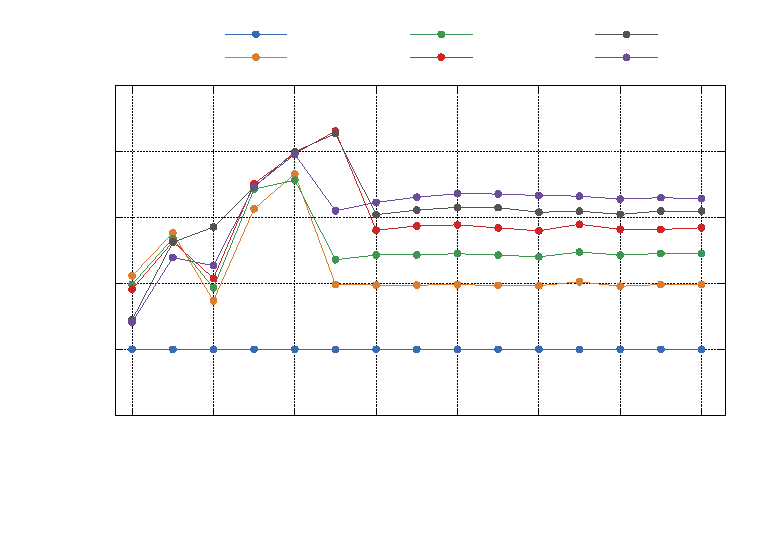
\includegraphics{BHMTSpeedup}}%
    \gplfronttext
  \end{picture}%
\endgroup
}
		\end{center}
	\end{frame}

	\begin{frame}{Resultaten Barnes-Hut Multithread: Strong scaling}
		\begin{center}
			\resizebox{!}{.7\paperheight}{% GNUPLOT: LaTeX picture with Postscript
\begingroup
  % Encoding inside the plot.  In the header of your document, this encoding
  % should to defined, e.g., by using
  % \usepackage[cp1252,<other encodings>]{inputenc}
  \inputencoding{cp1252}%
  \makeatletter
  \providecommand\color[2][]{%
    \GenericError{(gnuplot) \space\space\space\@spaces}{%
      Package color not loaded in conjunction with
      terminal option `colourtext'%
    }{See the gnuplot documentation for explanation.%
    }{Either use 'blacktext' in gnuplot or load the package
      color.sty in LaTeX.}%
    \renewcommand\color[2][]{}%
  }%
  \providecommand\includegraphics[2][]{%
    \GenericError{(gnuplot) \space\space\space\@spaces}{%
      Package graphicx or graphics not loaded%
    }{See the gnuplot documentation for explanation.%
    }{The gnuplot epslatex terminal needs graphicx.sty or graphics.sty.}%
    \renewcommand\includegraphics[2][]{}%
  }%
  \providecommand\rotatebox[2]{#2}%
  \@ifundefined{ifGPcolor}{%
    \newif\ifGPcolor
    \GPcolorfalse
  }{}%
  \@ifundefined{ifGPblacktext}{%
    \newif\ifGPblacktext
    \GPblacktexttrue
  }{}%
  % define a \g@addto@macro without @ in the name:
  \let\gplgaddtomacro\g@addto@macro
  % define empty templates for all commands taking text:
  \gdef\gplbacktext{}%
  \gdef\gplfronttext{}%
  \makeatother
  \ifGPblacktext
    % no textcolor at all
    \def\colorrgb#1{}%
    \def\colorgray#1{}%
  \else
    % gray or color?
    \ifGPcolor
      \def\colorrgb#1{\color[rgb]{#1}}%
      \def\colorgray#1{\color[gray]{#1}}%
      \expandafter\def\csname LTw\endcsname{\color{white}}%
      \expandafter\def\csname LTb\endcsname{\color{black}}%
      \expandafter\def\csname LTa\endcsname{\color{black}}%
      \expandafter\def\csname LT0\endcsname{\color[rgb]{1,0,0}}%
      \expandafter\def\csname LT1\endcsname{\color[rgb]{0,1,0}}%
      \expandafter\def\csname LT2\endcsname{\color[rgb]{0,0,1}}%
      \expandafter\def\csname LT3\endcsname{\color[rgb]{1,0,1}}%
      \expandafter\def\csname LT4\endcsname{\color[rgb]{0,1,1}}%
      \expandafter\def\csname LT5\endcsname{\color[rgb]{1,1,0}}%
      \expandafter\def\csname LT6\endcsname{\color[rgb]{0,0,0}}%
      \expandafter\def\csname LT7\endcsname{\color[rgb]{1,0.3,0}}%
      \expandafter\def\csname LT8\endcsname{\color[rgb]{0.5,0.5,0.5}}%
    \else
      % gray
      \def\colorrgb#1{\color{black}}%
      \def\colorgray#1{\color[gray]{#1}}%
      \expandafter\def\csname LTw\endcsname{\color{white}}%
      \expandafter\def\csname LTb\endcsname{\color{black}}%
      \expandafter\def\csname LTa\endcsname{\color{black}}%
      \expandafter\def\csname LT0\endcsname{\color{black}}%
      \expandafter\def\csname LT1\endcsname{\color{black}}%
      \expandafter\def\csname LT2\endcsname{\color{black}}%
      \expandafter\def\csname LT3\endcsname{\color{black}}%
      \expandafter\def\csname LT4\endcsname{\color{black}}%
      \expandafter\def\csname LT5\endcsname{\color{black}}%
      \expandafter\def\csname LT6\endcsname{\color{black}}%
      \expandafter\def\csname LT7\endcsname{\color{black}}%
      \expandafter\def\csname LT8\endcsname{\color{black}}%
    \fi
  \fi
    \setlength{\unitlength}{0.0500bp}%
    \ifx\gptboxheight\undefined%
      \newlength{\gptboxheight}%
      \newlength{\gptboxwidth}%
      \newsavebox{\gptboxtext}%
    \fi%
    \setlength{\fboxrule}{0.5pt}%
    \setlength{\fboxsep}{1pt}%
\begin{picture}(7200.00,5040.00)%
    \gplgaddtomacro\gplbacktext{%
      \csname LTb\endcsname%%
      \put(814,704){\makebox(0,0)[r]{\strut{}$0$}}%
      \csname LTb\endcsname%%
      \put(814,1332){\makebox(0,0)[r]{\strut{}$0.2$}}%
      \csname LTb\endcsname%%
      \put(814,1960){\makebox(0,0)[r]{\strut{}$0.4$}}%
      \csname LTb\endcsname%%
      \put(814,2589){\makebox(0,0)[r]{\strut{}$0.6$}}%
      \csname LTb\endcsname%%
      \put(814,3217){\makebox(0,0)[r]{\strut{}$0.8$}}%
      \csname LTb\endcsname%%
      \put(814,3845){\makebox(0,0)[r]{\strut{}$1$}}%
      \csname LTb\endcsname%%
      \put(946,484){\makebox(0,0){\strut{}$1$}}%
      \csname LTb\endcsname%%
      \put(2117,484){\makebox(0,0){\strut{}$2$}}%
      \csname LTb\endcsname%%
      \put(3289,484){\makebox(0,0){\strut{}$3$}}%
      \csname LTb\endcsname%%
      \put(4460,484){\makebox(0,0){\strut{}$4$}}%
      \csname LTb\endcsname%%
      \put(5632,484){\makebox(0,0){\strut{}$5$}}%
      \csname LTb\endcsname%%
      \put(6803,484){\makebox(0,0){\strut{}$6$}}%
    }%
    \gplgaddtomacro\gplfronttext{%
      \csname LTb\endcsname%%
      \put(396,2431){\rotatebox{-270}{\makebox(0,0){\strut{}effici\"entie}}}%
      \put(3874,154){\makebox(0,0){\strut{}# cores}}%
      \csname LTb\endcsname%%
      \put(2794,4867){\makebox(0,0)[r]{\strut{}4096 bodies}}%
      \csname LTb\endcsname%%
      \put(2794,4647){\makebox(0,0)[r]{\strut{}16384 bodies}}%
      \csname LTb\endcsname%%
      \put(2794,4427){\makebox(0,0)[r]{\strut{}65536 bodies}}%
      \csname LTb\endcsname%%
      \put(5497,4867){\makebox(0,0)[r]{\strut{}262144 bodies}}%
      \csname LTb\endcsname%%
      \put(5497,4647){\makebox(0,0)[r]{\strut{}1048576 bodies}}%
    }%
    \gplbacktext
    \put(0,0){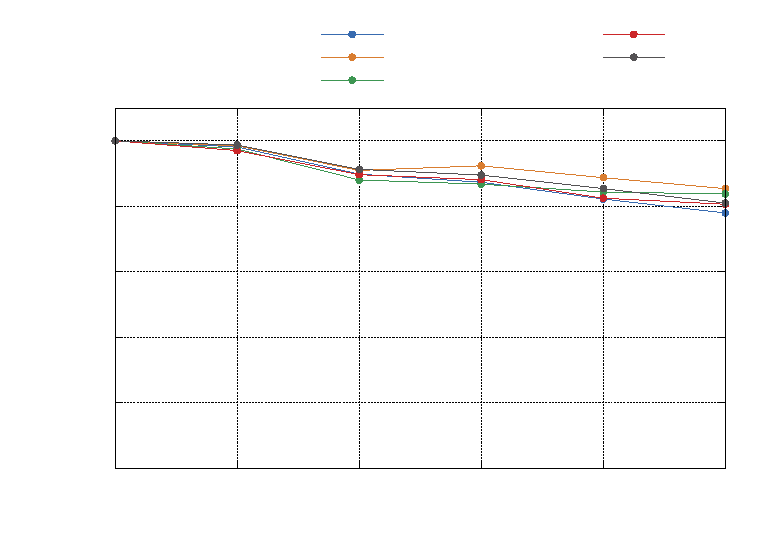
\includegraphics{BHStrong}}%
    \gplfronttext
  \end{picture}%
\endgroup
}
		\end{center}
	\end{frame}

	\begin{frame}{Resultaten Barnes-Hut GPU: Speedup (slowdown)}
		\begin{center}
			\resizebox{!}{.7\paperheight}{% GNUPLOT: LaTeX picture with Postscript
\begingroup
  % Encoding inside the plot.  In the header of your document, this encoding
  % should to defined, e.g., by using
  % \usepackage[cp1252,<other encodings>]{inputenc}
  \inputencoding{cp1252}%
  \makeatletter
  \providecommand\color[2][]{%
    \GenericError{(gnuplot) \space\space\space\@spaces}{%
      Package color not loaded in conjunction with
      terminal option `colourtext'%
    }{See the gnuplot documentation for explanation.%
    }{Either use 'blacktext' in gnuplot or load the package
      color.sty in LaTeX.}%
    \renewcommand\color[2][]{}%
  }%
  \providecommand\includegraphics[2][]{%
    \GenericError{(gnuplot) \space\space\space\@spaces}{%
      Package graphicx or graphics not loaded%
    }{See the gnuplot documentation for explanation.%
    }{The gnuplot epslatex terminal needs graphicx.sty or graphics.sty.}%
    \renewcommand\includegraphics[2][]{}%
  }%
  \providecommand\rotatebox[2]{#2}%
  \@ifundefined{ifGPcolor}{%
    \newif\ifGPcolor
    \GPcolorfalse
  }{}%
  \@ifundefined{ifGPblacktext}{%
    \newif\ifGPblacktext
    \GPblacktexttrue
  }{}%
  % define a \g@addto@macro without @ in the name:
  \let\gplgaddtomacro\g@addto@macro
  % define empty templates for all commands taking text:
  \gdef\gplbacktext{}%
  \gdef\gplfronttext{}%
  \makeatother
  \ifGPblacktext
    % no textcolor at all
    \def\colorrgb#1{}%
    \def\colorgray#1{}%
  \else
    % gray or color?
    \ifGPcolor
      \def\colorrgb#1{\color[rgb]{#1}}%
      \def\colorgray#1{\color[gray]{#1}}%
      \expandafter\def\csname LTw\endcsname{\color{white}}%
      \expandafter\def\csname LTb\endcsname{\color{black}}%
      \expandafter\def\csname LTa\endcsname{\color{black}}%
      \expandafter\def\csname LT0\endcsname{\color[rgb]{1,0,0}}%
      \expandafter\def\csname LT1\endcsname{\color[rgb]{0,1,0}}%
      \expandafter\def\csname LT2\endcsname{\color[rgb]{0,0,1}}%
      \expandafter\def\csname LT3\endcsname{\color[rgb]{1,0,1}}%
      \expandafter\def\csname LT4\endcsname{\color[rgb]{0,1,1}}%
      \expandafter\def\csname LT5\endcsname{\color[rgb]{1,1,0}}%
      \expandafter\def\csname LT6\endcsname{\color[rgb]{0,0,0}}%
      \expandafter\def\csname LT7\endcsname{\color[rgb]{1,0.3,0}}%
      \expandafter\def\csname LT8\endcsname{\color[rgb]{0.5,0.5,0.5}}%
    \else
      % gray
      \def\colorrgb#1{\color{black}}%
      \def\colorgray#1{\color[gray]{#1}}%
      \expandafter\def\csname LTw\endcsname{\color{white}}%
      \expandafter\def\csname LTb\endcsname{\color{black}}%
      \expandafter\def\csname LTa\endcsname{\color{black}}%
      \expandafter\def\csname LT0\endcsname{\color{black}}%
      \expandafter\def\csname LT1\endcsname{\color{black}}%
      \expandafter\def\csname LT2\endcsname{\color{black}}%
      \expandafter\def\csname LT3\endcsname{\color{black}}%
      \expandafter\def\csname LT4\endcsname{\color{black}}%
      \expandafter\def\csname LT5\endcsname{\color{black}}%
      \expandafter\def\csname LT6\endcsname{\color{black}}%
      \expandafter\def\csname LT7\endcsname{\color{black}}%
      \expandafter\def\csname LT8\endcsname{\color{black}}%
    \fi
  \fi
    \setlength{\unitlength}{0.0500bp}%
    \ifx\gptboxheight\undefined%
      \newlength{\gptboxheight}%
      \newlength{\gptboxwidth}%
      \newsavebox{\gptboxtext}%
    \fi%
    \setlength{\fboxrule}{0.5pt}%
    \setlength{\fboxsep}{1pt}%
\begin{picture}(7200.00,5040.00)%
    \gplgaddtomacro\gplbacktext{%
      \csname LTb\endcsname%%
      \put(1606,1209){\makebox(0,0)[r]{\strut{}$0.0078125$}}%
      \csname LTb\endcsname%%
      \put(1606,1656){\makebox(0,0)[r]{\strut{}$0.015625$}}%
      \csname LTb\endcsname%%
      \put(1606,2103){\makebox(0,0)[r]{\strut{}$0.03125$}}%
      \csname LTb\endcsname%%
      \put(1606,2550){\makebox(0,0)[r]{\strut{}$0.0625$}}%
      \csname LTb\endcsname%%
      \put(1606,2997){\makebox(0,0)[r]{\strut{}$0.125$}}%
      \csname LTb\endcsname%%
      \put(1606,3444){\makebox(0,0)[r]{\strut{}$0.25$}}%
      \csname LTb\endcsname%%
      \put(1606,3891){\makebox(0,0)[r]{\strut{}$0.5$}}%
      \csname LTb\endcsname%%
      \put(1606,4338){\makebox(0,0)[r]{\strut{}$1$}}%
      \csname LTb\endcsname%%
      \put(1878,1077){\rotatebox{-30}{\makebox(0,0)[l]{\strut{}$64$}}}%
      \csname LTb\endcsname%%
      \put(2553,1077){\rotatebox{-30}{\makebox(0,0)[l]{\strut{}$256$}}}%
      \csname LTb\endcsname%%
      \put(3229,1077){\rotatebox{-30}{\makebox(0,0)[l]{\strut{}$1024$}}}%
      \csname LTb\endcsname%%
      \put(3904,1077){\rotatebox{-30}{\makebox(0,0)[l]{\strut{}$4096$}}}%
      \csname LTb\endcsname%%
      \put(4579,1077){\rotatebox{-30}{\makebox(0,0)[l]{\strut{}$16384$}}}%
      \csname LTb\endcsname%%
      \put(5255,1077){\rotatebox{-30}{\makebox(0,0)[l]{\strut{}$65536$}}}%
      \csname LTb\endcsname%%
      \put(5930,1077){\rotatebox{-30}{\makebox(0,0)[l]{\strut{}$262144$}}}%
      \csname LTb\endcsname%%
      \put(6605,1077){\rotatebox{-30}{\makebox(0,0)[l]{\strut{}$1.04858\times10^{6}$}}}%
    }%
    \gplgaddtomacro\gplfronttext{%
      \csname LTb\endcsname%%
      \put(396,2904){\rotatebox{-270}{\makebox(0,0){\strut{}Speedup}}}%
      \put(4270,154){\makebox(0,0){\strut{}# bodies}}%
      \csname LTb\endcsname%%
      \put(3982,4867){\makebox(0,0)[r]{\strut{}Single thread CPU}}%
      \csname LTb\endcsname%%
      \put(7081,4867){\makebox(0,0)[r]{\strut{}GPU Offload}}%
    }%
    \gplbacktext
    \put(0,0){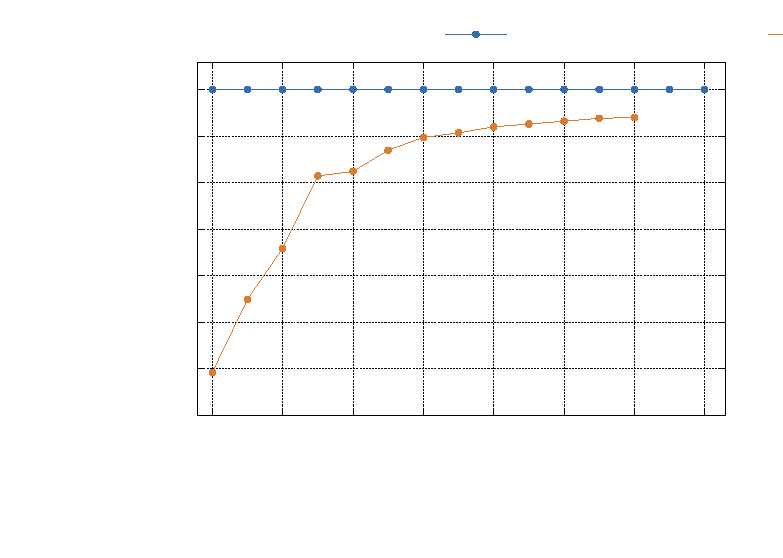
\includegraphics{BHOSpeedup}}%
    \gplfronttext
  \end{picture}%
\endgroup
}
		\end{center}
	\end{frame}

	\begin{frame}{Resultaten Barnes-Hut Recursief}
		\begin{center}
			\resizebox{!}{.7\paperheight}{% GNUPLOT: LaTeX picture with Postscript
\begingroup
  % Encoding inside the plot.  In the header of your document, this encoding
  % should to defined, e.g., by using
  % \usepackage[cp1252,<other encodings>]{inputenc}
  \inputencoding{cp1252}%
  \makeatletter
  \providecommand\color[2][]{%
    \GenericError{(gnuplot) \space\space\space\@spaces}{%
      Package color not loaded in conjunction with
      terminal option `colourtext'%
    }{See the gnuplot documentation for explanation.%
    }{Either use 'blacktext' in gnuplot or load the package
      color.sty in LaTeX.}%
    \renewcommand\color[2][]{}%
  }%
  \providecommand\includegraphics[2][]{%
    \GenericError{(gnuplot) \space\space\space\@spaces}{%
      Package graphicx or graphics not loaded%
    }{See the gnuplot documentation for explanation.%
    }{The gnuplot epslatex terminal needs graphicx.sty or graphics.sty.}%
    \renewcommand\includegraphics[2][]{}%
  }%
  \providecommand\rotatebox[2]{#2}%
  \@ifundefined{ifGPcolor}{%
    \newif\ifGPcolor
    \GPcolorfalse
  }{}%
  \@ifundefined{ifGPblacktext}{%
    \newif\ifGPblacktext
    \GPblacktexttrue
  }{}%
  % define a \g@addto@macro without @ in the name:
  \let\gplgaddtomacro\g@addto@macro
  % define empty templates for all commands taking text:
  \gdef\gplbacktext{}%
  \gdef\gplfronttext{}%
  \makeatother
  \ifGPblacktext
    % no textcolor at all
    \def\colorrgb#1{}%
    \def\colorgray#1{}%
  \else
    % gray or color?
    \ifGPcolor
      \def\colorrgb#1{\color[rgb]{#1}}%
      \def\colorgray#1{\color[gray]{#1}}%
      \expandafter\def\csname LTw\endcsname{\color{white}}%
      \expandafter\def\csname LTb\endcsname{\color{black}}%
      \expandafter\def\csname LTa\endcsname{\color{black}}%
      \expandafter\def\csname LT0\endcsname{\color[rgb]{1,0,0}}%
      \expandafter\def\csname LT1\endcsname{\color[rgb]{0,1,0}}%
      \expandafter\def\csname LT2\endcsname{\color[rgb]{0,0,1}}%
      \expandafter\def\csname LT3\endcsname{\color[rgb]{1,0,1}}%
      \expandafter\def\csname LT4\endcsname{\color[rgb]{0,1,1}}%
      \expandafter\def\csname LT5\endcsname{\color[rgb]{1,1,0}}%
      \expandafter\def\csname LT6\endcsname{\color[rgb]{0,0,0}}%
      \expandafter\def\csname LT7\endcsname{\color[rgb]{1,0.3,0}}%
      \expandafter\def\csname LT8\endcsname{\color[rgb]{0.5,0.5,0.5}}%
    \else
      % gray
      \def\colorrgb#1{\color{black}}%
      \def\colorgray#1{\color[gray]{#1}}%
      \expandafter\def\csname LTw\endcsname{\color{white}}%
      \expandafter\def\csname LTb\endcsname{\color{black}}%
      \expandafter\def\csname LTa\endcsname{\color{black}}%
      \expandafter\def\csname LT0\endcsname{\color{black}}%
      \expandafter\def\csname LT1\endcsname{\color{black}}%
      \expandafter\def\csname LT2\endcsname{\color{black}}%
      \expandafter\def\csname LT3\endcsname{\color{black}}%
      \expandafter\def\csname LT4\endcsname{\color{black}}%
      \expandafter\def\csname LT5\endcsname{\color{black}}%
      \expandafter\def\csname LT6\endcsname{\color{black}}%
      \expandafter\def\csname LT7\endcsname{\color{black}}%
      \expandafter\def\csname LT8\endcsname{\color{black}}%
    \fi
  \fi
    \setlength{\unitlength}{0.0500bp}%
    \ifx\gptboxheight\undefined%
      \newlength{\gptboxheight}%
      \newlength{\gptboxwidth}%
      \newsavebox{\gptboxtext}%
    \fi%
    \setlength{\fboxrule}{0.5pt}%
    \setlength{\fboxsep}{1pt}%
\begin{picture}(7200.00,5040.00)%
    \gplgaddtomacro\gplbacktext{%
      \csname LTb\endcsname%%
      \put(1606,704){\makebox(0,0)[r]{\strut{}$0.0078125$}}%
      \csname LTb\endcsname%%
      \put(1606,1218){\makebox(0,0)[r]{\strut{}$0.015625$}}%
      \csname LTb\endcsname%%
      \put(1606,1731){\makebox(0,0)[r]{\strut{}$0.03125$}}%
      \csname LTb\endcsname%%
      \put(1606,2245){\makebox(0,0)[r]{\strut{}$0.0625$}}%
      \csname LTb\endcsname%%
      \put(1606,2758){\makebox(0,0)[r]{\strut{}$0.125$}}%
      \csname LTb\endcsname%%
      \put(1606,3272){\makebox(0,0)[r]{\strut{}$0.25$}}%
      \csname LTb\endcsname%%
      \put(1606,3785){\makebox(0,0)[r]{\strut{}$0.5$}}%
      \csname LTb\endcsname%%
      \put(1606,4299){\makebox(0,0)[r]{\strut{}$1$}}%
      \csname LTb\endcsname%%
      \put(1878,484){\makebox(0,0){\strut{}$64$}}%
      \csname LTb\endcsname%%
      \put(2553,484){\makebox(0,0){\strut{}$256$}}%
      \csname LTb\endcsname%%
      \put(3229,484){\makebox(0,0){\strut{}$1024$}}%
      \csname LTb\endcsname%%
      \put(3904,484){\makebox(0,0){\strut{}$4096$}}%
      \csname LTb\endcsname%%
      \put(4579,484){\makebox(0,0){\strut{}$16384$}}%
      \csname LTb\endcsname%%
      \put(5255,484){\makebox(0,0){\strut{}$65536$}}%
      \csname LTb\endcsname%%
      \put(5930,484){\makebox(0,0){\strut{}$262144$}}%
      \csname LTb\endcsname%%
      \put(6605,484){\makebox(0,0){\strut{}$1.04858\times10^{6}$}}%
    }%
    \gplgaddtomacro\gplfronttext{%
      \csname LTb\endcsname%%
      \put(396,2651){\rotatebox{-270}{\makebox(0,0){\strut{}Speedup}}}%
      \put(4270,154){\makebox(0,0){\strut{}# bodies}}%
      \csname LTb\endcsname%%
      \put(3982,4867){\makebox(0,0)[r]{\strut{}Single thread CPU}}%
      \csname LTb\endcsname%%
      \put(7081,4867){\makebox(0,0)[r]{\strut{}GPU Offload}}%
    }%
    \gplbacktext
    \put(0,0){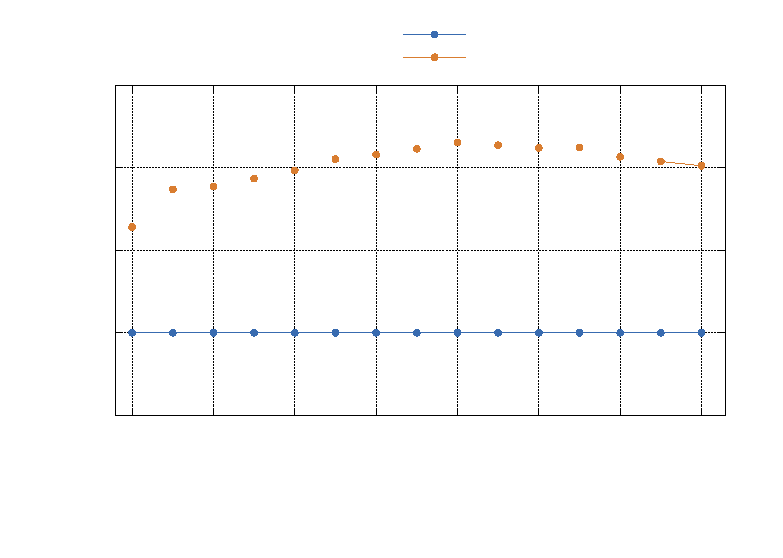
\includegraphics{BHTSpeedup}}%
    \gplfronttext
  \end{picture}%
\endgroup
}
		\end{center}
	\end{frame}
	
	\begin{frame}{Resultaat van simulatie}
		\begin{center}
%			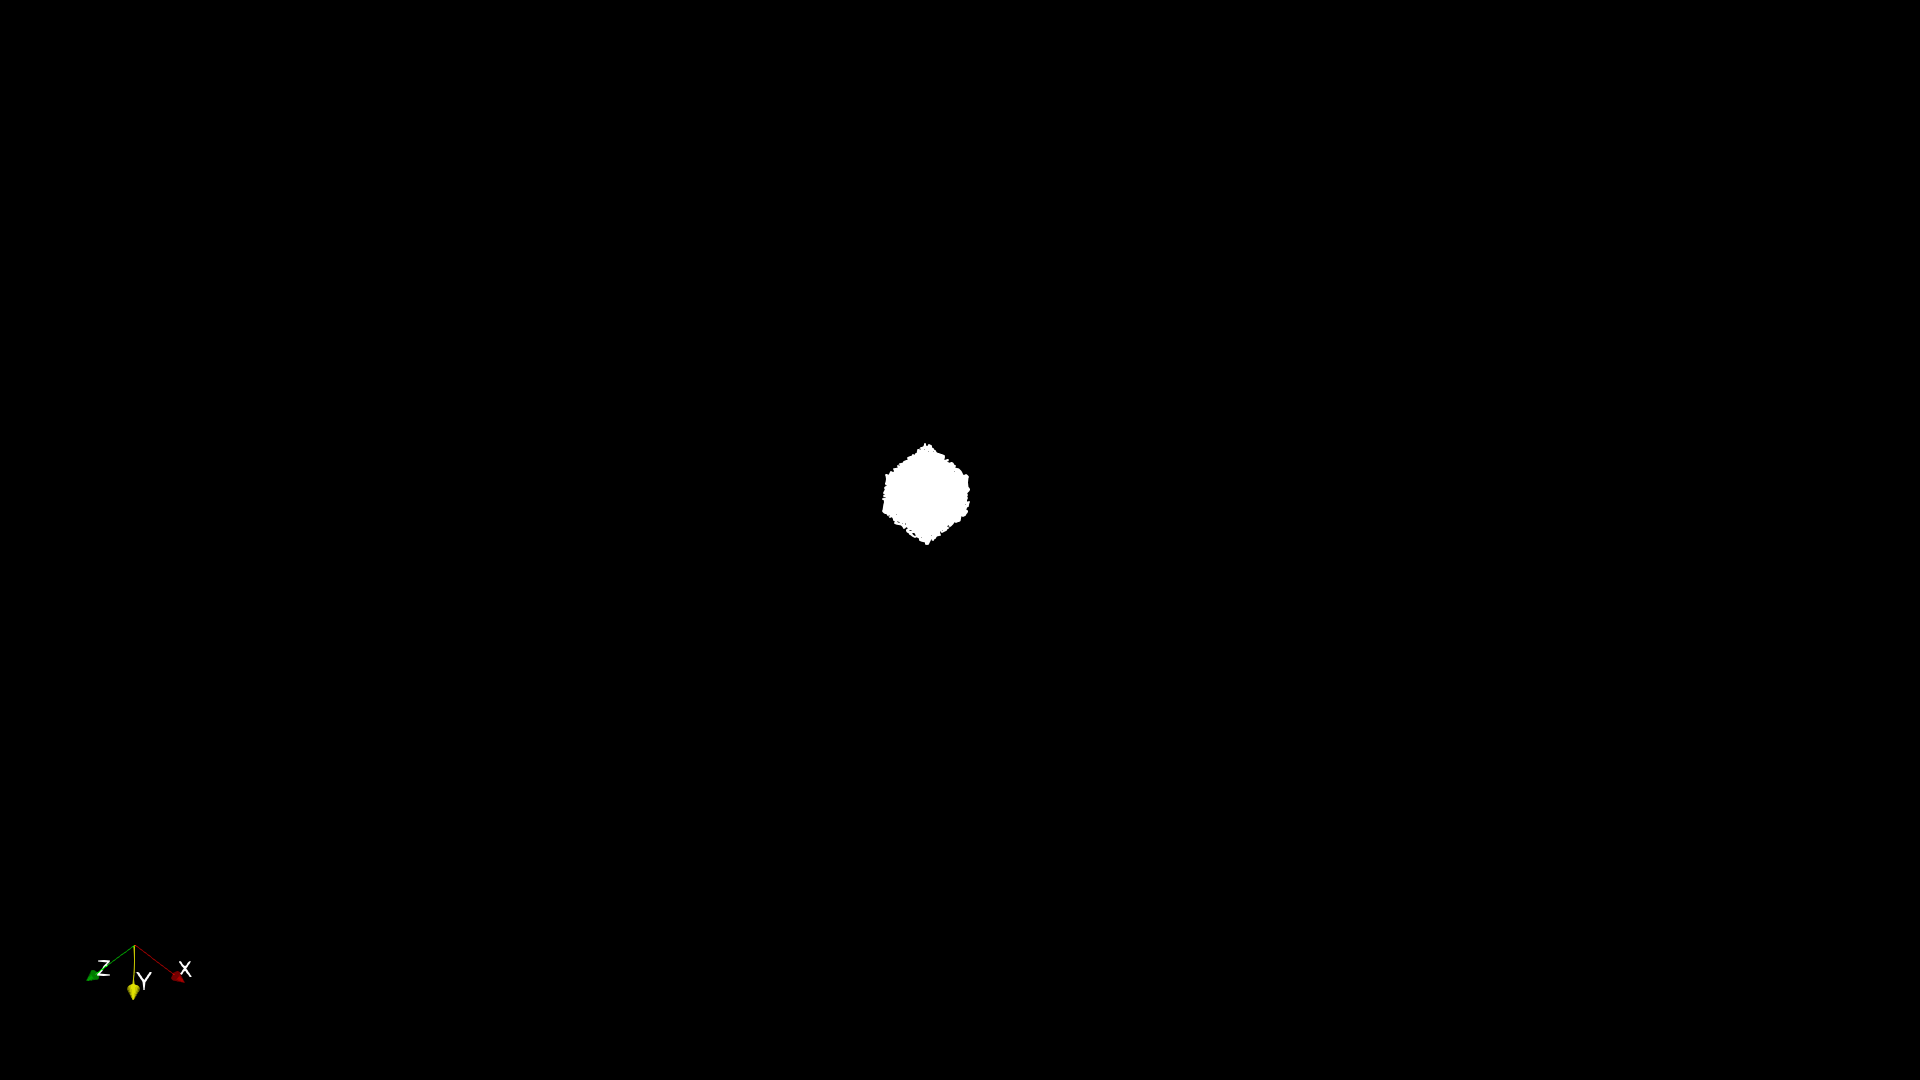
\includegraphics[width=0.8\linewidth]{out.png}
%			\movie{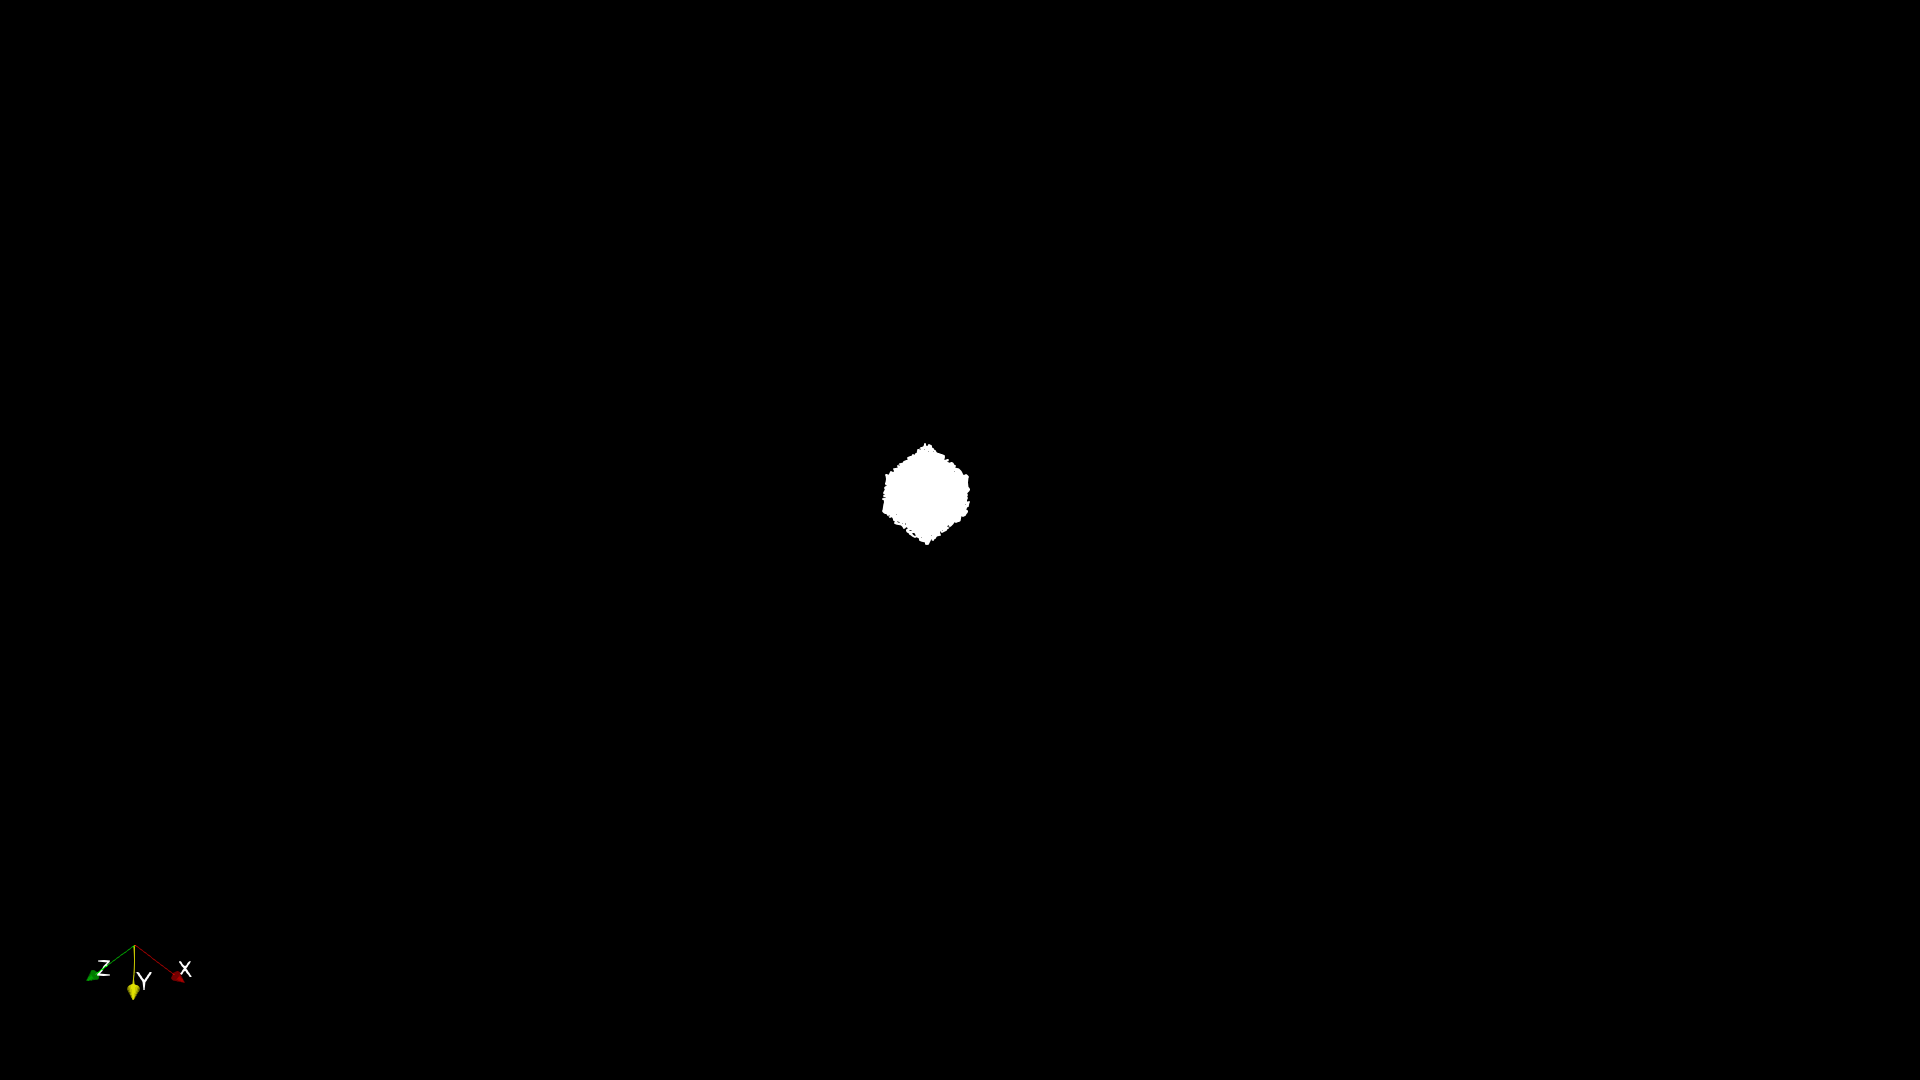
\includegraphics[width=0.8\linewidth]{out.png}}{out2.ogv}
		\end{center}
	\end{frame}
	
	\begin{frame}{Einde}
		\begin{center}
			Nog vragen?
		\end{center}
	\end{frame}
	
\end{document}

